\documentclass[tikz,border=12pt]{standalone}
\usepackage[T1]{fontenc}
\usepackage{mathpazo}
\usepackage{amsmath,amssymb}
\usetikzlibrary{arrows.meta, positioning, calc, fit, decorations.pathreplacing}
\definecolor{stblue}{HTML}{7B97AD}
\definecolor{rwgold}{HTML}{B8995E}
\definecolor{sage}{HTML}{7A9A7E}
\definecolor{dkbrown}{HTML}{3D3530}
\definecolor{wmgray}{HTML}{7B7067}
\definecolor{cream}{HTML}{F9F6F0}
\definecolor{border}{HTML}{D4C9B8}
\definecolor{terracotta}{HTML}{C47A6A}
\definecolor{lavender}{HTML}{907EA0}

\begin{document}
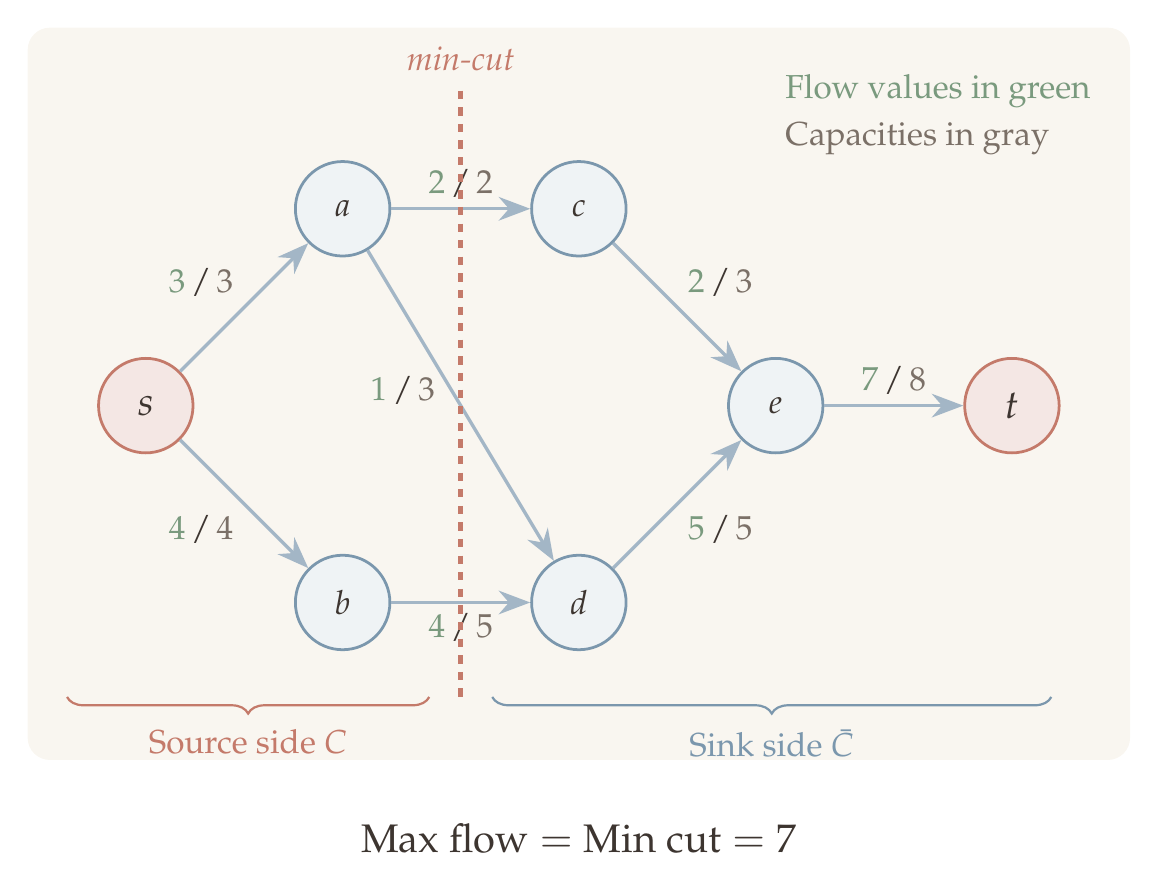
\begin{tikzpicture}[
    >={Stealth[length=4mm, width=3mm]},
    every node/.style={text=dkbrown},
    node distance=2cm and 2.5cm,
    bg/.style={fill=cream},
  ]

  % Background
  \fill[cream, rounded corners=8pt] (-1.5,-3.5) rectangle (12.5,5.8);

  % Nodes
  \node[circle, fill=terracotta!18, draw=terracotta, line width=1pt,
        minimum size=1.2cm, font=\Large\bfseries] (s) at (0,1) {$s$};
  \node[circle, fill=stblue!12, draw=stblue, line width=1pt,
        minimum size=1.2cm, font=\large] (a) at (2.5,3.5) {$a$};
  \node[circle, fill=stblue!12, draw=stblue, line width=1pt,
        minimum size=1.2cm, font=\large] (b) at (2.5,-1.5) {$b$};
  \node[circle, fill=stblue!12, draw=stblue, line width=1pt,
        minimum size=1.2cm, font=\large] (c) at (5.5,3.5) {$c$};
  \node[circle, fill=stblue!12, draw=stblue, line width=1pt,
        minimum size=1.2cm, font=\large] (d) at (5.5,-1.5) {$d$};
  \node[circle, fill=stblue!12, draw=stblue, line width=1pt,
        minimum size=1.2cm, font=\large] (e) at (8.0,1) {$e$};
  \node[circle, fill=terracotta!18, draw=terracotta, line width=1pt,
        minimum size=1.2cm, font=\Large\bfseries] (t) at (11.0,1) {$t$};

  % Edge style
  \tikzset{
    flowedge/.style={->, line width=1.2pt, stblue!70},
  }

  % Edges with flow/capacity labels
  \draw[flowedge] (s) -- (a)
    node[midway, above left, font=\large] {%
      \textcolor{sage}{3}\,/\,\textcolor{wmgray}{3}};

  \draw[flowedge] (s) -- (b)
    node[midway, below left, font=\large] {%
      \textcolor{sage}{4}\,/\,\textcolor{wmgray}{4}};

  \draw[flowedge] (a) -- (c)
    node[midway, above, font=\large] {%
      \textcolor{sage}{2}\,/\,\textcolor{wmgray}{2}};

  \draw[flowedge] (a) -- (d)
    node[midway, left=2pt, font=\large, pos=0.45] {%
      \textcolor{sage}{1}\,/\,\textcolor{wmgray}{3}};

  \draw[flowedge] (b) -- (d)
    node[midway, below, font=\large] {%
      \textcolor{sage}{4}\,/\,\textcolor{wmgray}{5}};

  \draw[flowedge] (c) -- (e)
    node[midway, above right, font=\large] {%
      \textcolor{sage}{2}\,/\,\textcolor{wmgray}{3}};

  \draw[flowedge] (d) -- (e)
    node[midway, below right, font=\large] {%
      \textcolor{sage}{5}\,/\,\textcolor{wmgray}{5}};

  \draw[flowedge] (e) -- (t)
    node[midway, above, font=\large] {%
      \textcolor{sage}{7}\,/\,\textcolor{wmgray}{8}};

  % Min-cut dashed line
  \draw[terracotta, line width=1.8pt, dashed]
    (4.0, 5.0) -- (4.0, -2.8);

  % Cut label
  \node[font=\large\itshape, terracotta] at (4.0, 5.4) {min-cut};

  % Braces on source side
  \draw[decorate, decoration={brace, amplitude=6pt, mirror},
        terracotta, line width=0.8pt]
    (-1.0, -2.7) -- (3.6, -2.7)
    node[midway, below=8pt, font=\large, terracotta] {Source side $C$};

  % Braces on sink side
  \draw[decorate, decoration={brace, amplitude=6pt, mirror},
        stblue, line width=0.8pt]
    (4.4, -2.7) -- (11.5, -2.7)
    node[midway, below=8pt, font=\large, stblue] {Sink side $\bar{C}$};

  % Caption
  \node[font=\Large, text=dkbrown] at (5.5, -4.5)
    {$\text{Max flow} = \text{Min cut} = 7$};

  % Legend
  \node[font=\large, text=sage, anchor=west] at (8.0, 5.0)
    {Flow values in \textcolor{sage}{green}};
  \node[font=\large, text=wmgray, anchor=west] at (8.0, 4.4)
    {Capacities in \textcolor{wmgray}{gray}};

\end{tikzpicture}
\end{document}
